\documentclass[tikz,border=2pt]{standalone}
\usepackage{tikz}
\usetikzlibrary{arrows,positioning,shapes}
\begin{document}
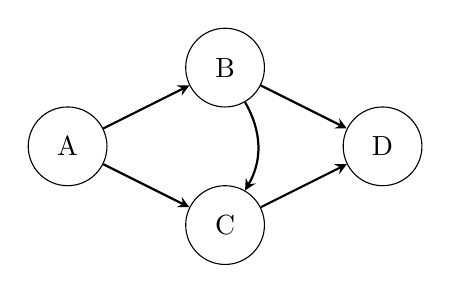
\begin{tikzpicture}[
    node/.style={circle, draw, minimum size=1cm},
    edge/.style={->, >=stealth, thick}
]
\node[node] (A) at (0,0) {A};
\node[node] (B) at (2,1) {B};
\node[node] (C) at (2,-1) {C};
\node[node] (D) at (4,0) {D};

\draw[edge] (A) -- (B);
\draw[edge] (A) -- (C);
\draw[edge] (B) -- (D);
\draw[edge] (C) -- (D);
\draw[edge, bend left] (B) to (C);
\end{tikzpicture}
\end{document}
